\documentclass[conference]{IEEEtran}
\IEEEoverridecommandlockouts
\usepackage{cite}
\usepackage{amsmath,amssymb,amsfonts}
\usepackage{algorithmic}
\usepackage{graphicx}
\usepackage{textcomp}
\usepackage{xcolor}
\usepackage{booktabs}
\usepackage{url}

\newcommand{\bl}[1]{\textcolor{blue}{#1}}
\newcommand{\re}[1]{\textcolor{orange}{#1}}


\graphicspath{{figures/}}

\def\BibTeX{{\rm B\kern-.05em{\sc i\kern-.025em b}\kern-.08em
    T\kern-.1667em\lower.7ex\hbox{E}\kern-.125emX}}

\begin{document}

\title{Learn To Tag - A Reinforcement Learning Environment with
Multi-Algorithm Agent Comparison and Human-in-the-Loop Training}

\author{%
\IEEEauthorblockN{ Ghanibhuti Gogoi}
\IEEEauthorblockA{\textit{HKUST GZ} \\
Student ID: 50014104 \\
ggogoi543@connect.hkust-gz.edu.cn.edu}
\and
\IEEEauthorblockN{ Siqi Chen}
\IEEEauthorblockA{\textit{HKUST GZ} \\
Student ID: 50012493 \\
schen972@connect.hkust-gz.edu.cn.edu}
\and
\IEEEauthorblockN{Yuhan Chen}
\IEEEauthorblockA{\textit{HKUST GZ} \\
Student ID: 50013198 \\
ychen590@connect.hkust-gz.edu.cn.edu}
}

\maketitle

\begin{abstract}
We study how the choice of reinforcement learning (RL) algorithm interacts
with the structure of the state space in a multi-agent tagging task. The
study is a $2{\times}2$ comparison: two algorithms covered in our course
(\re{tabular} Q-Learning and SARSA) and two exploratory algorithms (\re{deep} DQN and PPO) are each evaluated on
two tagging scenarios that differ only in their state representation. The
\emph{discrete} scenario is a $10{\times}10$ turn-based gridworld with one
tagger and one runner, in which the state is just the four integer
coordinates. The \emph{continuous} scenario is \textit{Learn To Tag}, a
full 2D Tag game we built in Pygame in which six agents move continuously
on a tile-based map, the tagger role transfers on every successful tag,
and each agent observes a 43-dimensional ego-centric vector of positions,
velocities, and wall raycasts. For the deep
methods \bl{(DQN and PPO)} we train two separate networks per algorithm---a tagger brain and a
runner brain---each trained only on the experiences of its own role, and
report performance per role. Every checkpoint is evaluated as an isolated
tagger (against random runners) and as an isolated runner (against a random
tagger), with head-to-head joint evaluation reported only for the discrete
scenario where \re{the two phases} of training make the head-to-head match-up
well defined. Our results separate cleanly along the two axes. In the
\emph{discrete} gridworld, all four algorithms train a near-perfect tagger
(98--99\% catch rate against a random runner) but the runner results split
sharply along on-policy/off-policy lines: SARSA's runner survives a trained
tagger 89\% of the time while Q-Learning's runner survives only 38\%, the
classical Cliff-Walking risk-profile contrast. The two deep methods
produce no runner that survives at all. In the \emph{continuous} full game,
the two tabular methods score exactly zero tags across 1000 training
epochs, while both deep methods learn: by the end of training DQN reaches
an isolated tagger score on the order of 40 tags per 2000-step episode and
PPO reaches a comparable level. The findings make explicit which algorithm--scenario pairs are
viable.
\end{abstract}

\begin{IEEEkeywords}
reinforcement learning, multi-agent systems, pursuit-evasion, role-switching,
deep Q-network, proximal policy optimization, reward shaping
\end{IEEEkeywords}

\section{Introduction}

\subsection{Problem Definition}

The reinforcement learning (RL) algorithms covered in this project span two
important axes. On one axis, they differ in how they represent the value
function: tabular methods (Q-Learning, SARSA) store one value per state,
while deep methods (DQN, PPO) approximate the value function with a neural
network. On the other axis, they differ in their update rule:
Q-Learning and DQN are off-policy and bootstrap from the maximum next-state
value, while SARSA and PPO are on-policy and bootstrap from the action that
will actually be taken. Standard textbook results state that tabular
methods are intended for finite, discrete state spaces, and that deep
methods are needed once the state becomes continuous or high-dimensional~\cite{sutton2018,mnih2015}.
But \emph{how much} does this matter in practice? On exactly the same task,
is the gap between tabular and deep methods small or catastrophic? And
within each family, does the off-policy/on-policy distinction produce a
visible behavioural difference?

We pose this as a concrete $2{\times}2$ study: four standard RL algorithms
$\times$ two tagging scenarios that differ only in the structure of the
state space.

\textbf{Discrete tagging scenario.} A $10{\times}10$ turn-based gridworld
with exactly one tagger and one runner. The state is the four integer
coordinates $(t_x, t_y, r_x, r_y)$, the action set is
$\{$stay, up, down, left, right$\}$, agents take alternating turns, and
each episode ends when the tagger reaches the runner's cell or after 200
turns. There are exactly $10^4$ states---small enough to be fully covered
by a Q-table.

\textbf{Continuous tagging scenario.} \textit{Learn To Tag}, a 2D Tag game
we built in Pygame. Six agents move \emph{continuously} on a tile-based
map at 30~Hz. One agent is the tagger; when it touches a runner, that
runner is respawned and becomes the new tagger. The game has no terminal
state. Each agent observes a 43-dimensional ego-centric vector containing
its own position and velocity, the relative offsets and distances of all
other active agents, eight wall-raycast distances, and a binary role flag.
The state space is continuous and effectively unbounded by tabular
standards.

The four algorithms (Q-Learning, SARSA, DQN, PPO) are evaluated on both
scenarios under identical reward design and identical evaluation
protocols. We expect the discrete scenario to be tractable for all four
algorithms (with possible behavioural differences between off-policy and
on-policy methods, predicted by the classical Cliff-Walking analysis~\cite{sutton2018}), and
the continuous scenario to be tractable only for the deep methods \re{(DIDN'T CHANGE. But can keep it like this if u think it's acceptable.)}. The
study makes both predictions falsifiable on the same code base.

\subsection{What We Built}

Beyond the two scenarios and the four algorithm implementations, the
project contains the integration glue needed to make a fair comparison:
\begin{enumerate}
    \item A single \texttt{BaseRLAlgorithm} interface that all four
    algorithms implement, so the menu can swap them without any other code
    changes.
    \item Two-brain training: every algorithm is trained as two
    independent networks, a tagger brain $\pi_T$ and a runner brain
    $\pi_R$. Each network is trained only on the experiences of its
    own role, so neither network sees contradictory chase-and-flee
    targets for the same observation. (A runtime wrapper that would
    route observations to the appropriate brain on every role flip was
    part of the original design, but the experiments reported here use
    the two networks as fixed-role policies; we revisit this in
    Section~\ref{sec:dualrole}.)
    \item A pure-proximity reward function with symmetric tagger and
    runner shaping. We arrived at this design after experimenting with
    several more elaborate reward functions, each of which produced a
    distinct behavioural pathology (Section~\ref{sec:reward}).
    \item A unified \texttt{run\_experiment.py} pipeline that trains any
    algorithm headlessly with periodic checkpoints and evaluates each
    checkpoint under isolated-role protocols (and a head-to-head joint
    protocol in the discrete scenario), producing training curves,
    role-trend plots, trajectory heatmaps, and rendered MP4 videos for
    qualitative behavioural inspection.
    \item A user-facing menu offering Player Mode (human + AI agents) and
    Simulation Mode (all AI), with the agents either continuing to learn
    in real time during play (\emph{Train Live}) or loading a pre-trained
    checkpoint (\emph{Use Trained}).
\end{enumerate}

We make no claim of novelty in the algorithms themselves; all four are
textbook implementations. The contribution is the controlled comparison: a
clean codebase where four standard RL algorithms can be trained, evaluated,
visualized, and compared on two scenarios that differ only in their state
structure.

\section{Literature Review}\label{sec:litreview}

Our problem---understanding how the choice of RL algorithm
interacts with the structure of the state space in a multi-agent
tagging task ---draws on six threads
of prior work: temporal-difference foundations, deep value-based RL,
policy-gradient and actor--critic methods, multi-agent reinforcement
learning, pursuit-evasion as a benchmark domain, and role/goal-conditional
policies. We survey each in turn and conclude with the gap our
$2{\times}2$ study addresses.

\subsection{Temporal-Difference Foundations}

The two tabular algorithms in our study, Q-Learning~\cite{watkins1989}
and SARSA~\cite{rummery1994}, are the canonical model-free
temporal-difference (TD) methods. Both estimate the action-value
function $Q(s,a)$ by repeatedly applying a sample-based Bellman
update. The two differ only in the bootstrap target: Q-Learning is
\emph{off-policy} and uses $\max_{a'} Q(s', a')$, while SARSA is
\emph{on-policy} and uses $Q(s', a')$ for the action $a'$ actually
taken next. The textbook treatment of Sutton and Barto~\cite{sutton2018}
establishes the convergence guarantees and limitations of both methods,
including the requirement of a finite, frequently-revisited state
space. Their Cliff-Walking example demonstrates a behavioural
consequence of the update-rule difference as professor taught in course. Q-Learning learns the aggressive optimal path along the cliff edge whereas SARSA learns a safer detour, because
SARSA's on-policy update accounts for the cost of exploratory actions
that an $\epsilon$-greedy policy will continue to take. Our Phase~2
gridworld result (SARSA runner: 89.4\% survival, Q-Learning runner:
38.1\%) reproduces this risk-profile asymmetry in a multi-agent
pursuit-evasion setting.

\subsection{Deep Value-Based Reinforcement Learning}

When the state space is continuous or high-dimensional, the central
operation of tabular RL becomes
infeasible, and function approximation is required. \textbf{DQN}
\cite{mnih2015} introduced a feed-forward neural network as the
approximator for $Q(s, a)$ on the Atari benchmark and stabilized
training with two key tricks: an experience replay buffer (which
decorrelates samples) and a periodically updated target network
(which stabilizes the bootstrap target). DQN's success on most of the 49 Atari games---triggered a wave of refinements: Double DQN~\cite{vanhasselt2016} addresses
the maximization bias of Q-Learning, Dueling DQN~\cite{wang2016}
factors the value into a state-value and an advantage stream, and
Rainbow~\cite{hessel2018} combines six such improvements into a
single state-of-the-art agent. Although our DQN implementation is the
original 2015 formulation, these refinements are immediate candidates
for follow-up work; we discuss this in Section~\ref{sec:conclusion}.

\subsection{Policy-Gradient and Actor--Critic Methods}

A complementary family of deep RL methods learns the policy
$\pi(a \mid s)$ directly through gradient ascent on the expected
return. The classical REINFORCE algorithm~\cite{williams1992}
introduced this idea in tabular form. Modern variants combine a
policy network (the \emph{actor}) with a learned value baseline
(the \emph{critic}) to reduce gradient variance. Trust-Region Policy
Optimization (TRPO)~\cite{schulman2015} bounded the size of each
policy update by an explicit KL-divergence constraint, and
\textbf{PPO}~\cite{schulman2017} replaced the constraint with a
simpler clipped surrogate objective that achieves comparable
performance with substantially less implementation complexity. PPO has become a de-facto standard for both single-agent control benchmarks and multi-agent simulation~\cite{yu2022}, partly because its on-policy updates rely on trajectories collected from the current policy, which can improve robustness and training stability in non-stationary environments compared with replay-buffer-based off-policy methods.

\subsection{Multi-Agent Reinforcement Learning}

Multi-agent RL (MARL) introduces several structural challenges that do
not arise in the single-agent case. The most fundamental is
\emph{non-stationarity}: from each agent's perspective, the
environment dynamics change as the other agents update their policies.
Several architectures address this. \textbf{MADDPG}~\cite{lowe2017}
extends DDPG with a centralized critic that observes all agents'
actions during training but a decentralized actor at execution time,
making the dynamics stationary from the critic's perspective.
\textbf{QMIX}~\cite{rashid2018} factorizes the joint value function
into per-agent value functions combined by a monotonic mixing network,
enabling decentralized execution while still providing centralized
training signals. \textbf{MAPPO}~\cite{yu2022} applies PPO to MARL
problems with a centralized value function and shows that PPO is, in
fact, surprisingly competitive with the more elaborate MARL methods on
the StarCraft Multi-Agent Challenge and other cooperative benchmarks.
The \textbf{PettingZoo} library~\cite{terry2021} consolidates the
multi-agent RL benchmark ecosystem analogously to OpenAI Gym for
single-agent RL. [to be deleted]

Our work also considers the challenges introduced by non-stationary
multi-agent environments, but focuses on an empirical comparison of how
different RL algorithms behave under these conditions rather than
proposing a new MARL coordination architecture. In particular, we study
the performance differences between classical tabular methods
(\textbf{Q-learning} and \textbf{SARSA}) and deep RL approaches
(\textbf{DQN} and \textbf{PPO}) in the symmetric two-agent Tag setting.
By evaluating both value-based and policy-based methods under the same
adversarial dynamics, we analyze how algorithmic design choices affect
training stability, adaptation, and final performance in non-stationary
multi-agent interaction.

\subsection{Pursuit-Evasion as an RL Benchmark}

Pursuit-evasion is a long-standing testbed for MARL because the rules
are simple but the behavioural space is rich. The most influential
recent example is OpenAI's Hide-and-Seek~\cite{baker2020}, in which
agents trained with PPO and self-play discovered emergent tool use
(block barricades, ramp manipulation) in a 3D physics simulator across
hundreds of millions of episodes. Pursuit-evasion has also been the
testbed for several robotics-flavoured studies in 2022--2023:
multi-UAV pursuit using Apollonius-circle geometry~\cite{liang2023},
and decentralized heterogeneous UAV swarms trained with
deep MARL~\cite{kouzeghar2023}. Cross-environment, the broader
self-play paradigm has produced human-level or super-human play in
Go (\textbf{AlphaGo Zero}~\cite{silver2017}), StarCraft~II
(\textbf{AlphaStar}~\cite{vinyals2019}), and Dota~2
(\textbf{OpenAI Five}~\cite{berner2019}).

A property shared by all of these benchmarks is that each agent's role
is \emph{fixed} for the entire episode (hider or seeker).

\subsection{Role-Conditional and Modular Policies}

Independently of the MARL literature, prior work has also explored how
RL agents can condition their behaviour on task- or goal-specific
context. \textbf{Universal Value Function Approximators}~\cite{schaul2015}
extend the value function with a goal variable $g$ and jointly learn
$V(s, g)$ across multiple goals, while \textbf{modular policy
networks}~\cite{andreas2017} decompose complex tasks into reusable
task-specific sub-policies guided by a higher-level policy structure.

Our setting can be viewed as a simplified binary-role instance of this
general idea. Rather than learning a single conditional policy
$\pi(a \mid s, g)$ shared across roles, we explicitly separate the two
opposing behaviours in Tag into distinct policies,
$\pi_T$ for the tagger and $\pi_R$ for the runner, and select between
them using a binary role flag. This design is motivated by the strongly
adversarial nature of the two roles, whose optimal behaviours differ
substantially.

\subsection{Comparative Studies and Empirical Benchmarks}

Despite the large body of work introducing individual RL algorithms,
systematic head-to-head comparisons across fundamentally different
algorithm families remain relatively limited. Benchmarks such as Atari
provided a common evaluation platform for deep value-based methods,
leading many subsequent studies to compare variants of the DQN
framework under standardized protocols. In contrast, comparisons across
the tabular-to-deep RL spectrum are less common, since classical
tabular methods are typically evaluated on small discrete state spaces
while deep RL methods are more often applied to high-dimensional
observations and continuous control tasks. Recent MARL benchmarks such
as MAPPO~\cite{yu2022} have extended this comparative philosophy to
multi-agent settings by evaluating PPO alongside methods such as QMIX
and MADDPG under shared cooperative environments.

Our work follows this comparative perspective. Rather than proposing a
new RL algorithm, we evaluate representatives from several major RL
families---\textbf{Q-Learning}, \textbf{SARSA}, \textbf{DQN}, and
\textbf{PPO}---under a unified experimental setting based on the same
Tag environment. This allows us to directly compare classical
tabular value-based methods, deep value-based methods, and policy
gradient methods under identical multi-agent interaction dynamics and
analyze how their underlying learning paradigms affect stability,
adaptation, and final performance in a non-stationary adversarial
setting.
\subsection{Research Gap}\label{sec:gap}

The literature surveyed above motivates three observations that
together define the gap our project addresses.

First, the textbook tells that tabular methods are confined to small
discrete domains while deep methods are needed for continuous ones
is treated as common knowledge but is rarely demonstrated empirically
on a single shared task. Our $2{\times}2$ design (four algorithms
$\times$ two scenarios that differ in state representation) makes
this claim verifiable on the same code base, with identical reward
function and evaluation protocol.

Second, the off-policy/on-policy distinction within the tabular family
(Q-Learning vs.\ SARSA) and within the deep family (DQN vs.\ PPO) is
known to produce different risk profiles in classical examples like
Cliff-Walking, but its consequences in a multi-agent pursuit-evasion
setting with dynamically changing roles are not, to our knowledge, characterized
in the literature. Our isolated-role evaluation
(Section~\ref{sec:eval-protocol}) allows us to analyze this effect more directly.


\section{System Description}\label{sec:system}

\subsection{Environment}

The Tag game is implemented as a 2D tile-based world built on Pygame. The
default map (\texttt{level\_small.txt}) is a 16$\times$11 grid (512$\times$352
pixels at \texttt{TILE\_SIZE}=32) containing six spawn points, four crate
spawns, and a single connected interior region with three doorways that
encourage navigation around obstacles. Six agents are spawned at random spawn
points each round; at any instant one is the tagger and five are runners.
When the tagger collides with a runner, the runner is teleported to a
randomly chosen spawn point and immediately becomes the new tagger. The game
runs at 60~FPS in rendered mode and at unbounded speed in headless mode for
training. Crates are pushable by entities and act as movable cover.

\subsection{Action Space}

Every agent shares the same discrete action space of size 5: no-op, up, down,
left, right. Diagonal movement is achieved by alternating actions between
decision frames. Decisions are made every \texttt{DECISION\_INTERVAL}=2 frames,
so an agent acts at 30~Hz; rewards accumulated between decisions are summed
into a single learning signal per decision step.

\subsection{Observation}\label{sec:obs}

We use a fixed-size 43-dimensional ego-centric observation vector
(Fig.~\ref{fig:observation}, Table~\ref{tab:obs}). Every position is
normalized either to $[0, 1]$ in the global frame or by the map's diagonal
length when expressed as a relative offset. Eliminated agents are filtered
out so that policies do not perceive or act upon inactive opponents. To give
the policy a sense of nearby geometry, we cast eight rays from the agent in
the cardinal and diagonal directions, each returning the normalized distance
to the nearest wall up to a maximum of eight tiles.

\begin{figure}[t]
\centerline{\includegraphics[width=0.95\columnwidth]{1.png}}
\caption{Ego-centric observation. The agent (green dot, centre) sees its
own position and velocity, the relative offset and distance to the
tagger (red) and the nearest runner (blue), and eight wall-raycast
distances (dashed amber). The right-hand panel lists the components
that make up the 43-dimensional vector.}
\label{fig:observation}
\end{figure}

\begin{table}[t]
\caption{Ego-Centric Observation (43 dimensions)}
\label{tab:obs}
\centering
\begin{tabular}{lcl}
\toprule
\textbf{Field} & \textbf{Dim} & \textbf{Description} \\
\midrule
self\_pos              & 2  & normalized $(x, y)$ position \\
self\_vel              & 2  & current velocity \\
is\_tagger             & 1  & role flag \\
tagger\_rel            & 2  & relative offset to tagger \\
tagger\_dist           & 1  & normalized distance to tagger \\
nearest\_runner\_rel   & 2  & relative offset to nearest runner \\
nearest\_runner\_dist  & 1  & normalized distance to nearest runner \\
wall\_rays             & 8  & 8-direction raycast distances \\
other\_agents          & 24 & up to 6 others $\times$ (rel\_pos, dist, role) \\
\bottomrule
\end{tabular}
\end{table}

\subsection{Modular Architecture}

The codebase is organized around a strict separation of concerns: \texttt{game/}
holds the simulation loop and tag rules; \texttt{entities/} defines the
\texttt{Player}, \texttt{Agent}, and \texttt{MovableObject} classes;
\texttt{world/} parses text-based maps; \texttt{physics/} handles AABB collision;
\texttt{rendering/} contains all Pygame draw calls and procedural sprite/texture
generation; and \texttt{rl/} contains the algorithm implementations and the
gym-like environment wrapper. Adding a new algorithm requires only
implementing the \texttt{BaseRLAlgorithm} abstract class and registering it in
\texttt{config.RL\_ALGORITHMS}.

\section{Methodology}
\subsection{Two-Brain Training}\label{sec:dualrole}

\begin{figure}[t]
\centerline{\includegraphics[width=0.95\columnwidth]{2.png}}
\caption{Two-brain training. For each algorithm we train two independent
networks: a tagger brain $\pi_T$ (chase policy, learned only from tagger
experiences) and a runner brain $\pi_R$ (flee policy, learned only from
runner experiences). The two networks never share gradients, so neither
sees contradictory chase-and-flee targets for the same observation.}
\label{fig:dualrole}
\end{figure}

As the objective of taggger and runner is opposite. Training a single network on both roles produces conflicting gradients: the same observation can demand opposite actions depending on whether the agent is currently the tagger or a runner. We avoid this conflict by training two completely separate networks per algorithm: a tagger brain
$\pi_T$ and a runner brain $\pi_R$ (Fig.~\ref{fig:dualrole}). $\pi_T$ is
trained only on tagger trajectories and $\pi_R$ only on runner
trajectories; their parameters and replay buffers are disjoint.

Our original design called for a runtime wrapper that would route every
observation to the appropriate brain by inspecting the
\texttt{is\_tagger} flag, so that an agent who tags a runner would
seamlessly switch from $\pi_R$ to $\pi_T$ on the next decision step. We
did not commit to this live-switching mechanism in the experiments
reported here. Instead, each network is trained and evaluated as a
fixed-role policy: in the discrete gridworld this is a clean fit (Phase
1 trains $\pi_T$, Phase 2 trains $\pi_R$, Phase 3 puts them head-to-head),
and in the continuous full game we report each brain's performance under
the isolated-role protocol of Section~\ref{sec:eval-protocol}. Live role
switching during play remains future work.

\subsection{Algorithms}\label{sec:algorithms}

All four algorithms inherit from \texttt{BaseRLAlgorithm} and implement
\texttt{select\_action(obs)}, \texttt{learn(s, a, r, s', done)}, and save/load.

\textbf{Q-Learning} discretizes each continuous observation field into between
4 and 9 bins, producing a hashable state key, and updates a Python dictionary
$Q\!:\!(s,a)\!\to\!\mathbb{R}$ with $\alpha=0.1$, $\gamma=0.95$, and
$\epsilon$-greedy exploration decaying from $1.0$ to $0.05$.

\textbf{SARSA} uses the same discretization but the on-policy update
$Q(s,a) \leftarrow Q(s,a) + \alpha\,(r + \gamma\,Q(s', a') - Q(s,a))$ where
$a'$ is the actual next action drawn from the policy.

\textbf{DQN} uses an MLP $Q_\theta(s, \cdot)$ that maps the 43-dimensional
observation to one Q-value per action, with experience replay (capacity 50k),
a target network synchronized every 500 gradient steps, the Adam optimizer
($\alpha=10^{-3}$), $\gamma=0.99$, and $\epsilon$ decaying linearly from
1.0 to 0.05 over the first 50k steps. The loss is the Huber loss between
$Q_\theta(s,a)$ and $r + \gamma \max_{a'} Q_{\theta^-}(s', a')$.

\textbf{PPO} uses a shared-trunk actor--critic network with two hidden layers
(128 units, ReLU). Trajectories are collected for 256 environment steps and
then optimized with the clipped surrogate objective ($\epsilon=0.2$) for four
epochs of mini-batch updates of size 64. We use generalized advantage
estimation ($\lambda=0.95$, $\gamma=0.99$), an entropy bonus ($0.01$) to
maintain exploration, and gradient clipping at norm 0.5.

\subsection{Reward Design}\label{sec:reward}

The reward function went through a long iterative debugging cycle that we
think is itself a useful course-project finding. Our first attempt used a
shaping term proportional to the \emph{absolute} distance between the
tagger and its nearest runner. This produced a clear bug: agents that were
already close to (or already far from) one another had no incentive to
move, because the per-frame reward was nearly identical whether they
stepped or not. We replaced absolute distance with a delta-based shaping
term (reward proportional to the change in distance from the previous
frame), which fixed the stationary-camping bug but introduced a new one:
agents learned to oscillate back-and-forth to farm small positive deltas.
We then enlarged the terminal tag reward so that successful tags (and
being-tagged penalties) dominated the return, added a time-scale schedule
to prevent early reward saturation, and added auxiliary terms for movement,
danger zone awareness, and anti-corner-camping. Each addition fixed one
behavioural pathology and introduced another.

We finally simplified back to a \emph{pure proximity} scheme that
satisfies three desiderata: (i) terminal events dominate, so policies
cannot gain by avoiding tag events; (ii) shaping is symmetric across
roles; and (iii) the gradient is silent at long range so that the policy
must learn navigation from the observation rather than from the reward.

Let $d$ denote the Euclidean distance between two agents and let
$R = 140$~pixels (approximately 4.4 tiles). The proximity term is
\begin{equation}
\phi(d) = c \cdot \max\!\left(0,\; 1 - \frac{d}{R}\right)^{2},
\quad c = 0.27.
\label{eq:phi}
\end{equation}
This is quadratic so the gradient is steepest near the tag zone where it
matters most, and zero outside the radius. The per-frame reward is (with
$i$ ranging over runners and $d_i$ the distance to runner $i$):
\begin{align}
r_{\text{tagger}} &=
    \begin{cases}
        +50 & \text{on tag,}\\
        -0.05 + \displaystyle\sum_{i} \phi(d_i) & \text{otherwise,}
    \end{cases}\\
r_{\text{runner}} &=
    \begin{cases}
        -80 & \text{on being tagged,}\\
        +0.10 - \phi(d_{\text{tagger}}) & \text{otherwise.}
    \end{cases}
\end{align}
The tag bonus and being-tagged penalty are intentionally asymmetric ($+50$
vs.\ $-80$) to push runners toward stronger caution than taggers' aggression.
Constant time pressure on the tagger ($-0.05$) and constant survival bonus
on the runner ($+0.10$) prevent both freezing and reward-farming.

\subsection{Training and Evaluation Pipeline}

A single script \texttt{run\_experiment.py} runs the entire workflow for any
algorithm. Training proceeds for a fixed number of epochs (each epoch is 2000
environment steps); two parallel headless simulations run in lock-step and
contribute experience to the two role-specific networks $\pi_T$ and $\pi_R$
(tagger experiences feed only $\pi_T$, runner experiences only $\pi_R$).
Checkpoints are saved at epochs $\{2, 5, 10, 50, 100\}$ for shorter runs
and additionally at $\{200, 500, 1000\}$ for longer runs, so that we can
characterize the full learning trajectory of each algorithm rather than
only its final state.

Each saved checkpoint is then evaluated under three protocols
(Section~\ref{sec:eval-protocol}). During evaluation an algorithm-level
\texttt{eval\_mode} flag is set so that learn updates are disabled and the
policy is truly frozen. A fixed random seed across algorithms ensures fair
cross-checkpoint comparison. The pipeline finally produces learning curves,
per-epoch performance bars, role-trend line plots, role-diagnostic plots,
trajectory overlays, and 2D position heatmaps.

\subsection{Evaluation Protocols}\label{sec:eval-protocol}

For each saved checkpoint, we measure two quantities in the
\emph{continuous full game}, each averaged over 20 evaluation episodes of
2000 steps:

\begin{itemize}
    \item \textbf{Isolated tagger evaluation:} the tagger brain is loaded
    but the runner brain is left untrained (random); higher tag counts
    indicate a stronger \emph{tagger}.
    \item \textbf{Isolated runner evaluation:} the runner brain is loaded
    but the tagger brain is random; \emph{lower} tag counts indicate
    stronger \emph{runners}.
\end{itemize}

A direct head-to-head match between the trained tagger brain and the
trained runner brain is not reported on the continuous full game because
the game has no terminal state and our two-brain policies do not switch
roles at runtime, so there is no well-defined ``joint policy'' to score.
We do report a head-to-head joint evaluation in the \emph{discrete}
gridworld, where each episode has a clean Phase-3 match-up of the
trained tagger vs.\ the trained runner of the same algorithm
(Section~\ref{sec:exp-grid}).

We additionally export rendered MP4 videos for the isolated and (in the
gridworld) joint evals so that emergent movement patterns
(corner-camping, wall-hugging escape, direct interception) can be
qualitatively recognized.

\section{Experiments}\label{sec:experiments}

This section describes the experimental design, such as the parameter setting, the parameters settings, and the evaluation protocol. All quantitative results, tables, figures, and interpretation appear in Section~\ref{sec:results}.

\subsection{Setup}

Inside each scenario, training and evaluation use identical observation,
reward, action space, and decision interval, so any cross-algorithm
difference is attributable to the algorithm itself. The continuous
scenario uses the default \texttt{level\_small} map and the
pure-proximity reward of Section~\ref{sec:reward}. The discrete scenario
uses the simpler step-based reward built into the gridworld environment
(small per-step shaping plus large terminal reward). All experiments run
on CPU.

\subsection{Continuous Full Game}\label{sec:exp-full}

We trained DQN, PPO, Q-Learning, and SARSA on the full Tag environment
for 1000 epochs each, where one epoch is 2000 environment steps and two
parallel headless simulations contribute experience per epoch. For each
algorithm we maintain two role-specific networks $\pi_T$ and $\pi_R$
(Section~\ref{sec:dualrole}); tagger experiences feed only $\pi_T$ and
runner experiences only $\pi_R$. We retain checkpoints at epochs
$\{2, 5, 10, 50, 100, 200, 500, 1000\}$ to trace the full learning
curve. Each checkpoint is evaluated under the isolated
tagger and isolated runner protocols of Section~\ref{sec:eval-protocol},
each averaged over 20 evaluation episodes of 2000 steps.

\subsection{Discrete Gridworld}\label{sec:exp-grid}

To compare the same four algorithms on a structurally simpler task, we
built a $10{\times}10$ turn-based gridworld with one tagger and one
runner. The state is just the four integer coordinates
$(t_x, t_y, r_x, r_y)$, the action set is the same five-action discrete
set used in the full game, and each episode terminates after 200 turns
or as soon as the tagger reaches the runner's cell. The total state
space is exactly $10^4$---tractable for a Q-table.

Each algorithm is trained in three phases:
\begin{itemize}
    \item \textbf{Phase 1 (5000 episodes).} Tagger trained against a
    randomly placed runner. Isolates the tagger learning problem.
    \item \textbf{Phase 2 (5000 episodes).} Runner trained against the
    same algorithm's frozen Phase-1 tagger. Isolates the runner
    learning problem against an already-strong opponent.
    \item \textbf{Phase 3 (200 episodes, no learning).} The trained
    tagger and trained runner of the same algorithm meet head-to-head.
    This is the head-to-head joint evaluation that the continuous game
    cannot support, since each phase produces a network that plays a
    fixed role for the entire episode.
\end{itemize}
We use the same training script across all four algorithms, with
algorithm-specific hyperparameters as listed in
Section~\ref{sec:algorithms}. Tabular methods use the same
$\epsilon$-greedy schedule as in the full game; deep methods use the
same network architecture and optimizer settings.

\section{Results and Discussion}\label{sec:results}

We report the continuous-game results first (Subsections A),
then the gridworld results
(Subsections B), qualitative
observations (Subsection C), and finally a synthesis
across the two scenarios (Subsection D).

\subsection{Continuous world setting}\label{sec:A}

\subsubsection{Tabular Methods Fail in the Continuous Game}\label{sec:res-tab-fail}
Q-Learning and SARSA produced \textbf{zero successful tags at every checkpoint} of the 1000-epoch full-game run (Fig.~\ref{fig:tabular-failure}, Table~\ref{tab:fullgame}). This means Q-learning and Sarsa do not learn the good policy in training.

Three factors combine to cause this. 
First, even after binning each of the 43 observation fields into 4--9 bins, the discretized state space contains many millions of cells, most of which a 1000-epoch run visits at most once.

Second, the game is continuing rather than episodic, so there is no stable terminal boundary that truncates temporal-difference backups. Q-learning and SARSA therefore rely on long-horizon bootstrapping under a non-stationary multi-agent environment, making value estimation unstable and slowing reward propagation.

Third, tabular methods cannot generalize across continuous state spaces: nearby states are treated as entirely independent entries in the Q-table, preventing knowledge learned in one region of the state space from transferring to similar states elsewhere. Section~\ref{sec:res-grid} shows that this limitation is structural rather than an implementation artifact.
 

\begin{figure*}[t]
\centerline{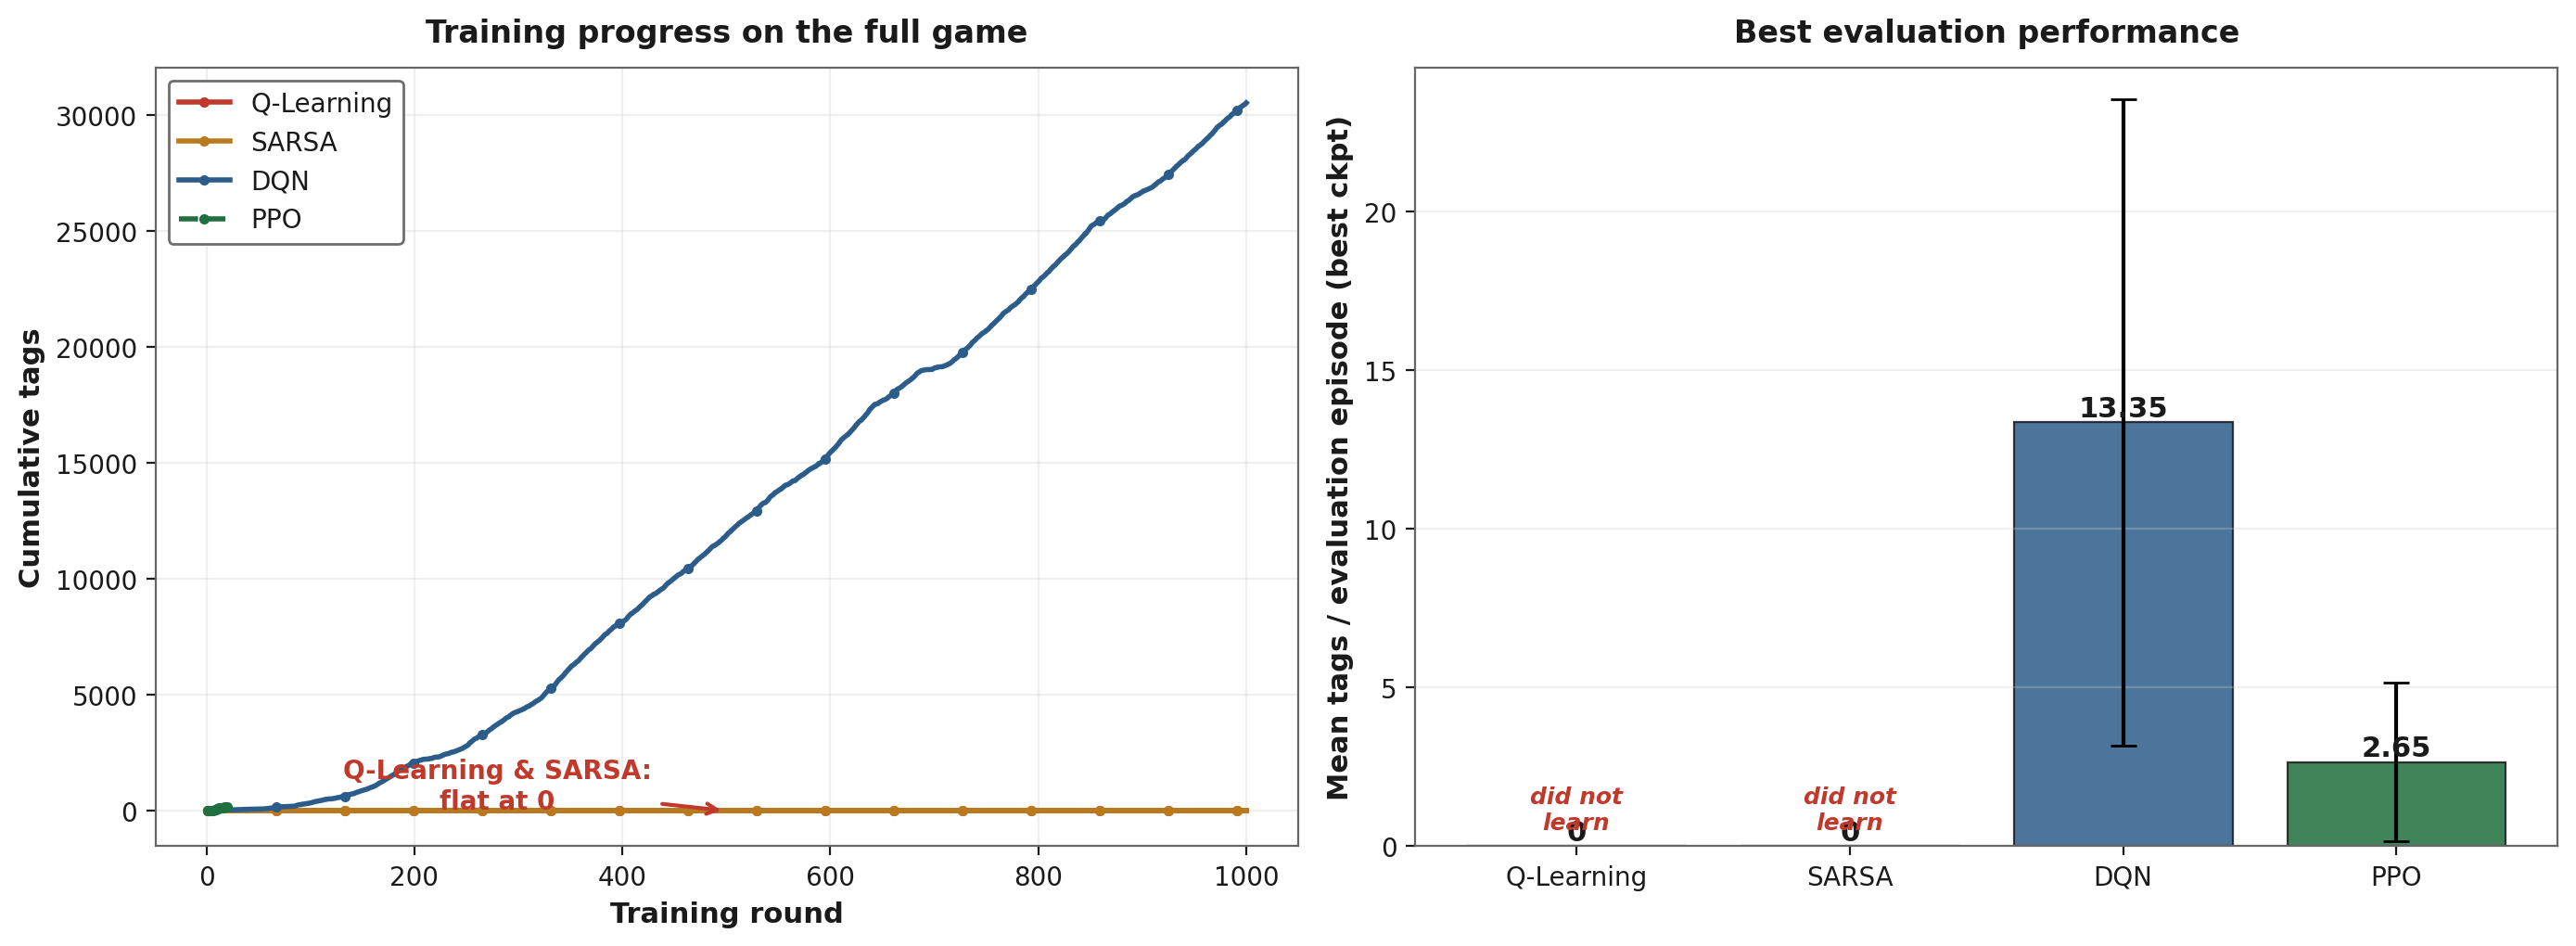
\includegraphics[width=0.92\textwidth]{tabular_failure.png}}
\caption{Algorithm comparison on the full Tag environment.
\textbf{Left:} cumulative tags over training rounds. \textbf{Right:} best
mean evaluation tag count per algorithm. }
\label{fig:tabular-failure}
\end{figure*}

\begin{table}[t]
\caption{Mean Tags per 2000-Step Evaluation Episode in the Continuous
Full Game (20 Episodes).}
\label{tab:fullgame}
\centering
\begin{tabular}{lccc}
\toprule
\textbf{Algorithm} & \textbf{Best epoch} & \textbf{Mean tags} & \textbf{Std} \\
\midrule
Q-Learning              & any           & 0.00            & 0.00 \\
SARSA                   & any           & 0.00            & 0.00 \\
DQN                    & 1000           & 41.85           & 0.00 \\
PPO (1000-epoch)        & 1000          & 30.30           & 5.42 \\
\bottomrule
\end{tabular}
\end{table}

\subsubsection{Deep Methods Learn the Continuous Game}\label{sec:res-deep}

Both DQN and PPO learn cleanly under the same training pipeline. The
DQN training curve (Fig.~\ref{fig:dqn-curve}) climbs sharply between
epochs 100 and 500, peaks around 13 mean tags near epoch 500, and
settles into a noisy plateau in the 10--13 range over the remaining
epochs. The PPO training curve (Fig.~\ref{fig:ppo-curve}) is markedly
higher: it rises rapidly between roughly epoch 200 and epoch 600 and
plateaus around 30 tags per episode. Both curves visibly plateau by
epoch 1000, suggesting that the budget is sufficient to reach a stable
policy in this environment.

\begin{figure}[t]
\centerline{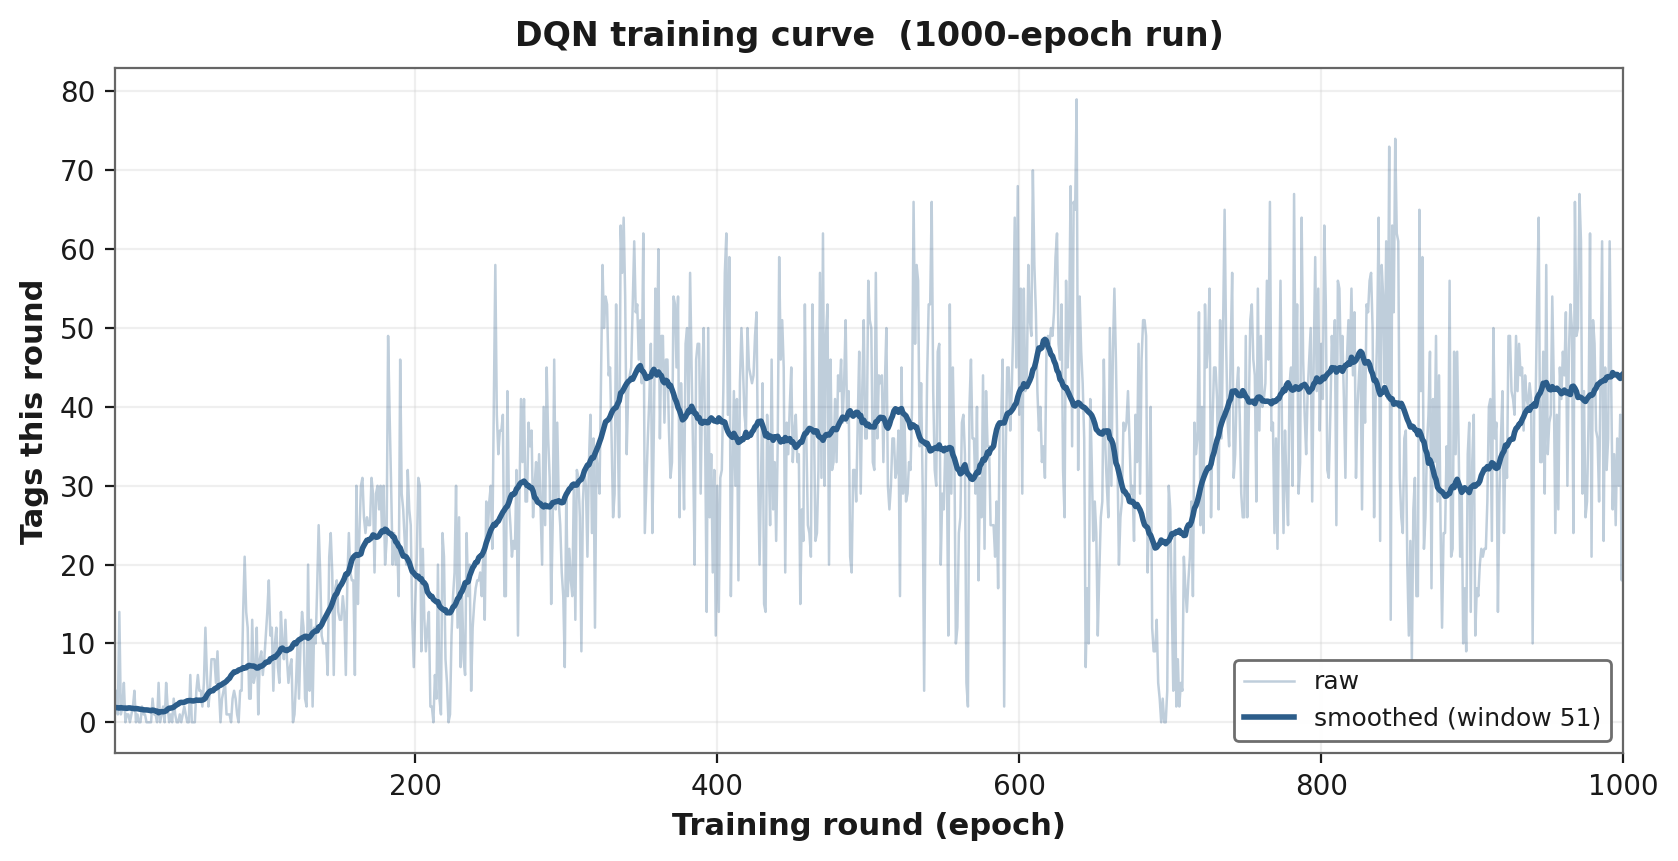
\includegraphics[width=0.95\columnwidth]{dqn_training_curve.png}}
\caption{DQN training curve over 1000 epochs.}
\label{fig:dqn-curve}
\end{figure}

\begin{figure}[t]
\centerline{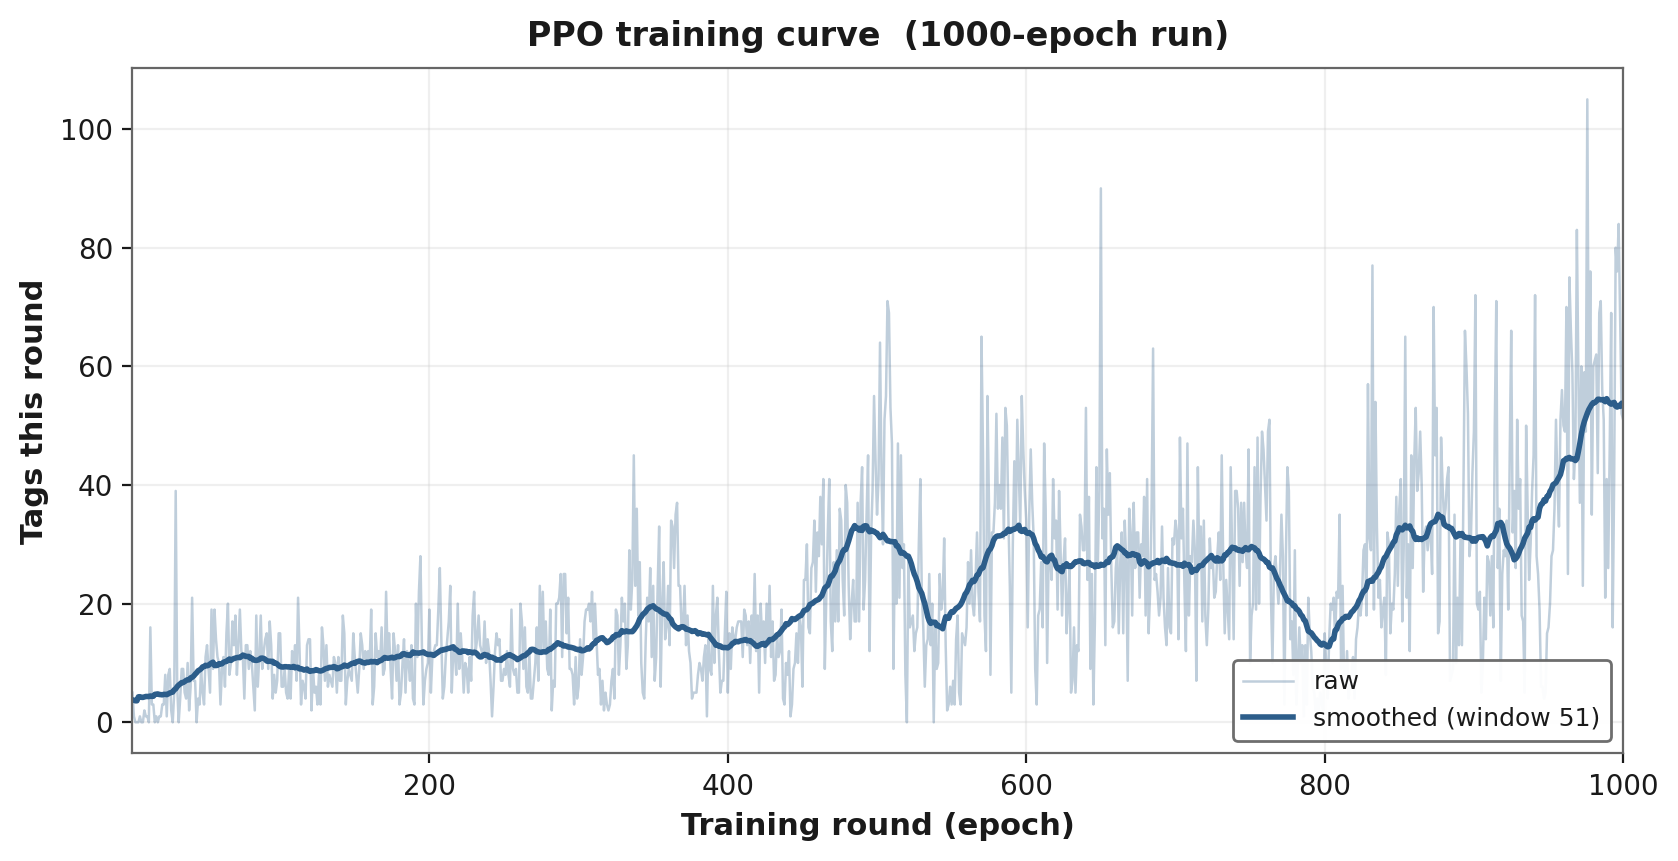
\includegraphics[width=0.95\columnwidth]{ppo_training_curve.png}}
\caption{PPO (1000-epoch) training curve over 1000 epochs.}
\label{fig:ppo-curve}
\end{figure}

\subsubsection{Isolated Role Evaluation Reveals a Tagger/Runner Asymmetry}\label{sec:res-iso}

The isolated-role protocol (Section~\ref{sec:eval-protocol}) lets us
measure the tagger brain $\pi_T$ and runner brain $\pi_R$ separately.
Table~\ref{tab:role} and Fig.~\ref{fig:role-eval} report DQN
across training; Table~\ref{tab:role-ppo} and Fig.~\ref{fig:pporole-eval}
report PPO under the same protocol. Two clear patterns emerge in both
algorithms.

\begin{figure}[t]
\centerline{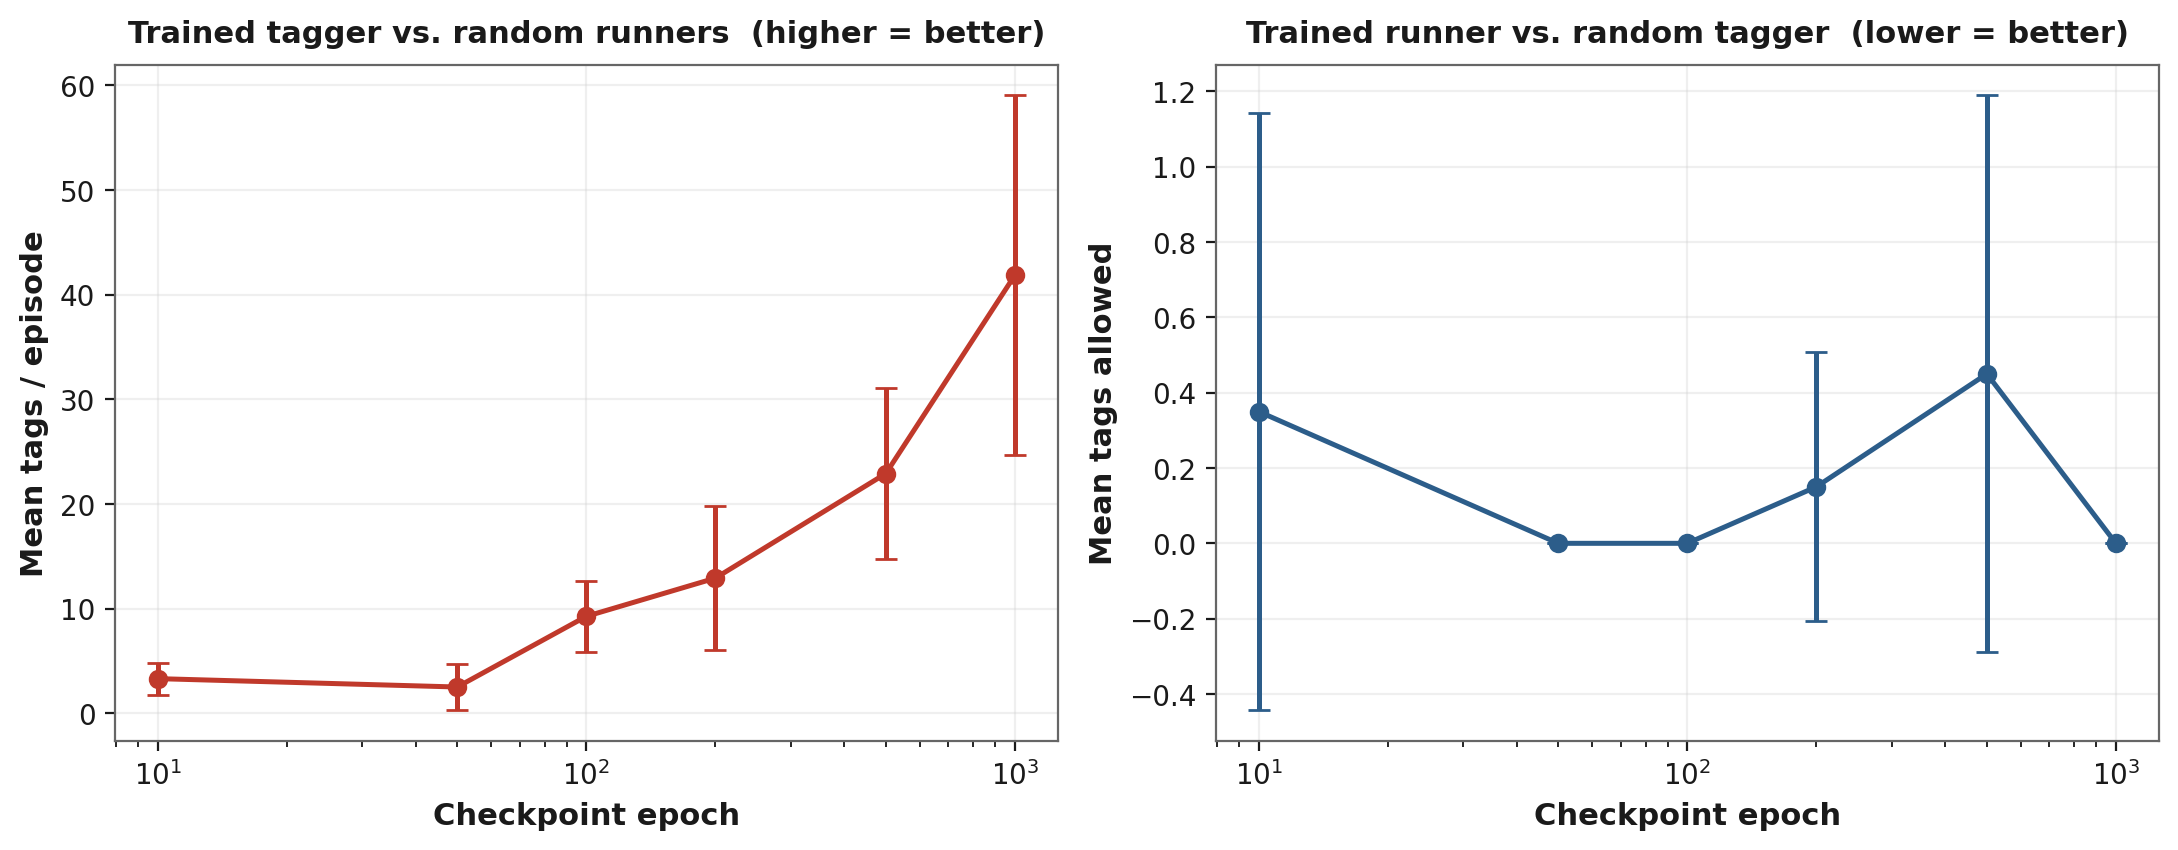
\includegraphics[width=0.95\columnwidth]{dqn_role_evaluation.png}}
\caption{Isolated role evaluation for DQN . Left: trained tagger
$\pi_T$ vs.\ random runners (higher = better tagger). Right: trained
runner $\pi_R$ vs.\ random tagger (lower = better runner).}
\label{fig:role-eval}
\end{figure}

\begin{figure}[t]
\centerline{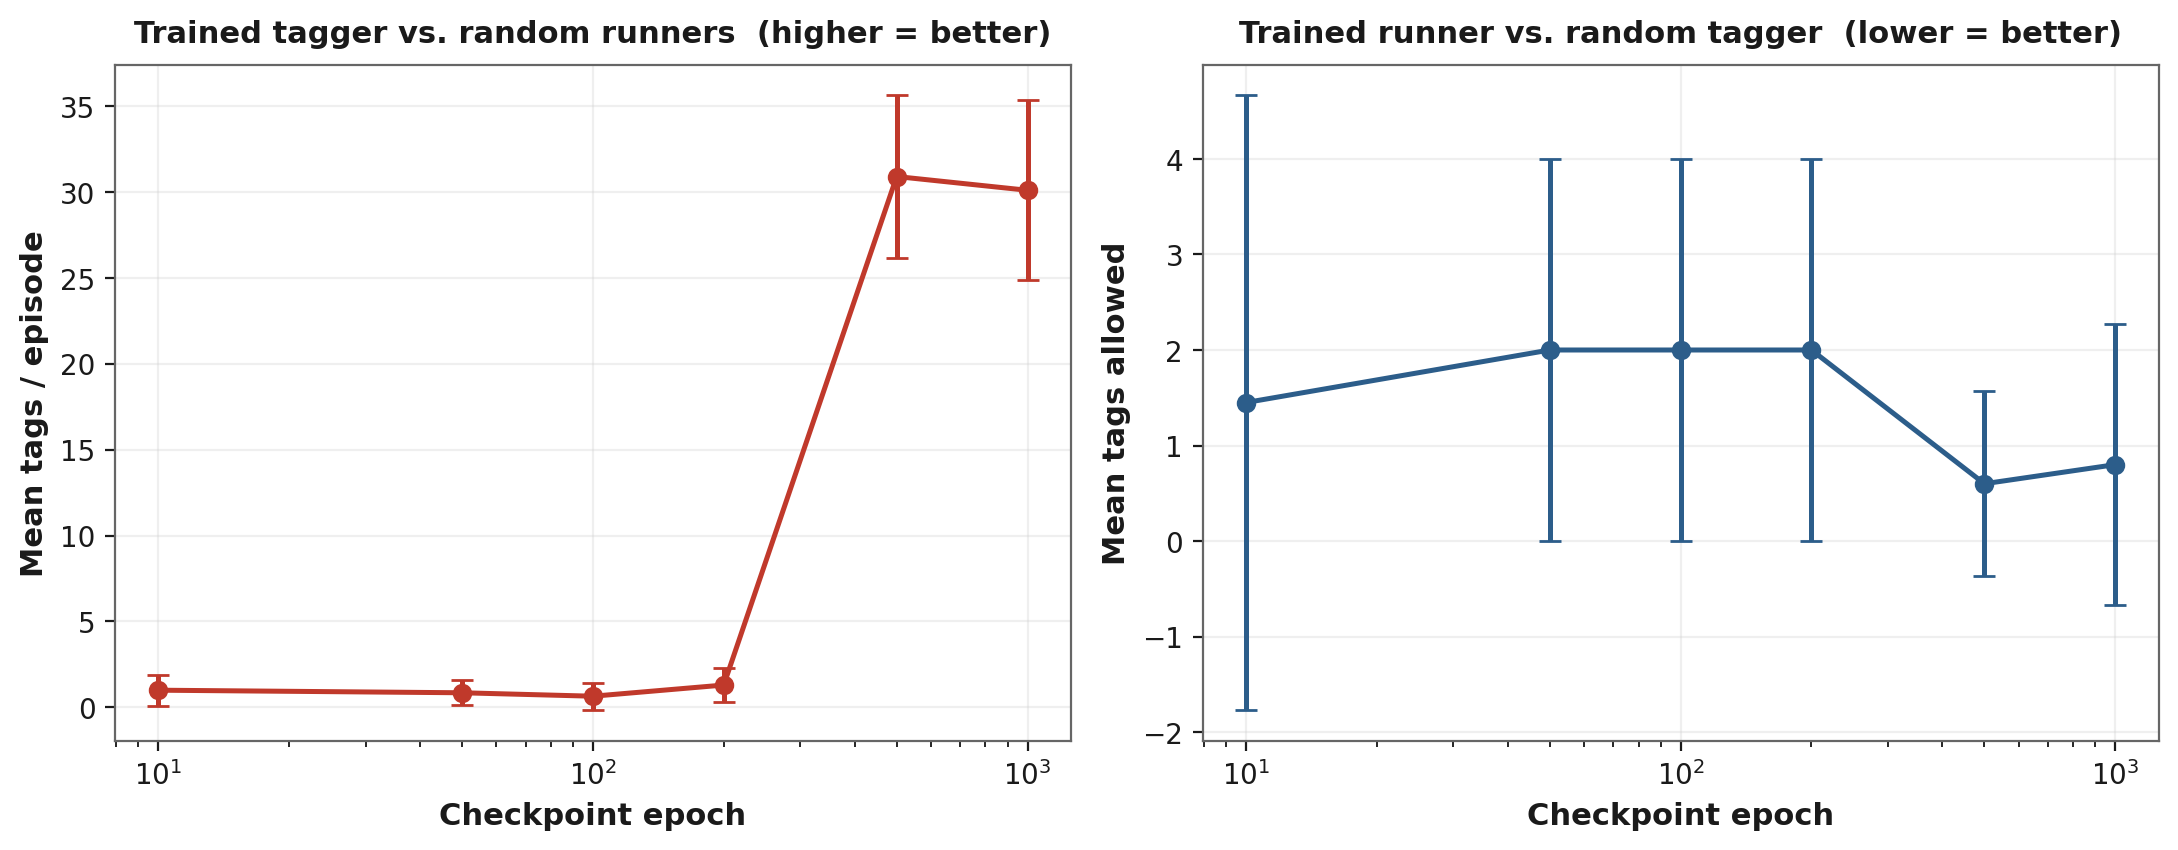
\includegraphics[width=0.95\columnwidth]{ppo_role_evaluation.png}}
\caption{Isolated role evaluation for PPO (1000-epoch run). Left:
trained tagger vs.\ random runners (higher is better tagger). Right:
trained runner vs.\ random tagger (lower is better runner).}
\label{fig:pporole-eval}
\end{figure}

\begin{table}[t]
\caption{Isolated Role Evaluation -- DQN}
\label{tab:role}
\centering
\begin{tabular}{lcc}
\toprule
\textbf{Epoch} & \textbf{Tagger tags} $\uparrow$ & \textbf{Runner tags} $\downarrow$ \\
\midrule
10   & 3.30  $\pm$ 1.52  & 0.35 $\pm$ 0.79 \\
50   & 2.50  $\pm$ 2.18  & 0.00 $\pm$ 0.00 \\
100  & 9.25  $\pm$ 3.37  & 0.00 $\pm$ 0.00 \\
200  & 12.90 $\pm$ 6.87  & 0.15 $\pm$ 0.36 \\
500  & 22.90 $\pm$ 8.16  & 0.45 $\pm$ 0.74 \\
1000 & \textbf{41.85 $\pm$ 17.19} & 0.00 $\pm$ 0.00 \\
\bottomrule
\end{tabular}
\end{table}

\begin{table}[t]
\caption{Isolated Role Evaluation -- PPO (1000-epoch run)}
\label{tab:role-ppo}
\centering
\begin{tabular}{lcc}
\toprule
\textbf{Epoch} & \textbf{Tagger tags} $\uparrow$ & \textbf{Runner tags} $\downarrow$ \\
\midrule
10   & 1.00  $\pm$ 0.89 & 1.45 $\pm$ 3.22 \\
50   & 0.85  $\pm$ 0.73 & 2.00 $\pm$ 2.00 \\
100  & 0.65  $\pm$ 0.79 & 2.00 $\pm$ 2.00 \\
200  & 1.30  $\pm$ 1.00 & 2.00 $\pm$ 2.00 \\
500  & 30.90 $\pm$ 4.73 & 0.60 $\pm$ 0.97 \\
1000 & 30.10 $\pm$ 5.23 & 0.80 $\pm$ 1.47 \\
\bottomrule
\end{tabular}
\end{table}

First, the tagger brain improves dramatically with training in both
algorithms. DQN climbs from 3.30 tags at epoch 10 to 41.85 tags at
epoch 1000 against a random opponent. PPO is even more abrupt: it stays near zero through epoch 200 and then jumps to 30.90 tags at epoch 500. 

Second, the runner brain remains very strong in both algorithms (DQN $\le 0.65$, PPO $\le 2.0$ tags allowed): a random tagger almost never catches the trained runners. This is excellent
runner performance in absolute terms but partially reflects the
weakness of a random tagger rather than rapid learning of the runner.

The asymmetry has two implications. First, separating tagger and runner evaluations is essential: aggregate performance metrics would misleadingly suggest balanced improvement across both roles, whereas the observed gains arise primarily from the tagger policy while the runner policy remains comparatively stable. Second, the
sharp PPO transition between epochs 200 and 500 (Table~\ref{tab:role-ppo})
is qualitatively different from DQN's smoother climb (Table~\ref{tab:role}),
suggesting that PPO's clipped policy update produces a phase-transition
style improvement in this environment, while DQN's incremental Q-value
updates produce a steadier climb.

\subsection{Discrete world setting}\label{sec:B}

\subsubsection{Tabular Methods Recover in the Gridworld}\label{sec:res-grid}

The same four algorithms run on the $10{\times}10$ gridworld behave
very differently. Table~\ref{tab:gridworld-all} reports the full
Phase~1/2/3 results.

\begin{table}[t]
\caption{Gridworld Evaluation -- All Four Algorithms.}
\label{tab:gridworld-all}
\centering
\begin{tabular}{lccc}
\toprule
              & \textbf{Phase 1} & \textbf{Phase 2}     & \textbf{Phase 3} \\
              & tagger vs.\ rand. & runner vs.\ trained & head-to-head    \\
\textbf{Algo} & catch rate $\uparrow$ & survival $\uparrow$ & catch / avg steps \\
\midrule
Q-Learning  & 100.0\%   & 38.14\%             & 62.5\% / 81.3        \\
SARSA       & 100.0\%   & 89.40\%             & 9.0\%  / 182.7       \\
DQN         & 99.50\%   & \textbf{96.60\%}    & \textbf{3.4\% / 193.2} \\
PPO         & 99.30\%   & 0.00\%              & 100.0\% / 9.1        \\
\bottomrule
\end{tabular}
\end{table}

\textbf{Phase 1 (tagger vs.\ random runner).} All four algorithms learn
near-perfect taggers. The two tabular methods reach 100\% catch rate;
DQN and PPO are within one percentage point. The deep methods do not
lose any quality from their neural function approximation, and the
tabular methods solve the chase task exactly as the textbook predicts.
The top row of Fig.~\ref{fig:tabular-training-curves} shows the tabular
convergence: both Q-Learning and SARSA climb from $\sim$70\% to a 100\%
rolling catch rate within roughly 1000 episodes and remain there for
the remaining 4000.

\textbf{Phase 2 (runner vs.\ frozen trained tagger).} For each
algorithm, the runner is trained against the same algorithm's frozen
Phase-1 tagger. The four algorithms split into three regimes. DQN,
with its 50k-transition replay buffer, produces the strongest runner
of the four (96.6\% greedy-eval survival against the frozen Phase-1
DQN tagger). SARSA is second (89.4\%) and Q-Learning is a distant
third (38.1\%); we interpret the SARSA/Q-Learning gap in
Subsection~\ref{sec:res-cliff}. PPO, run with the same network
architecture, learning rate, and 5000-episode budget as DQN, fails
entirely (0\% survival): its runner is caught in essentially every
evaluation episode. The bottom row of
Fig.~\ref{fig:tabular-training-curves} shows the tabular divergence
during training: with the tagger frozen and $\epsilon$ still decaying,
the SARSA runner's rolling survival rate climbs to roughly 50\% by
5000 episodes, while the Q-Learning runner stays below 5\% for the
entire run. The DQN--PPO gap, despite identical capacity and
hyperparameters, is the central new finding of this revision: it
isolates a sample-efficiency effect that we discuss in
Subsection~\ref{sec:res-synth}.

\begin{figure}[t]
\centerline{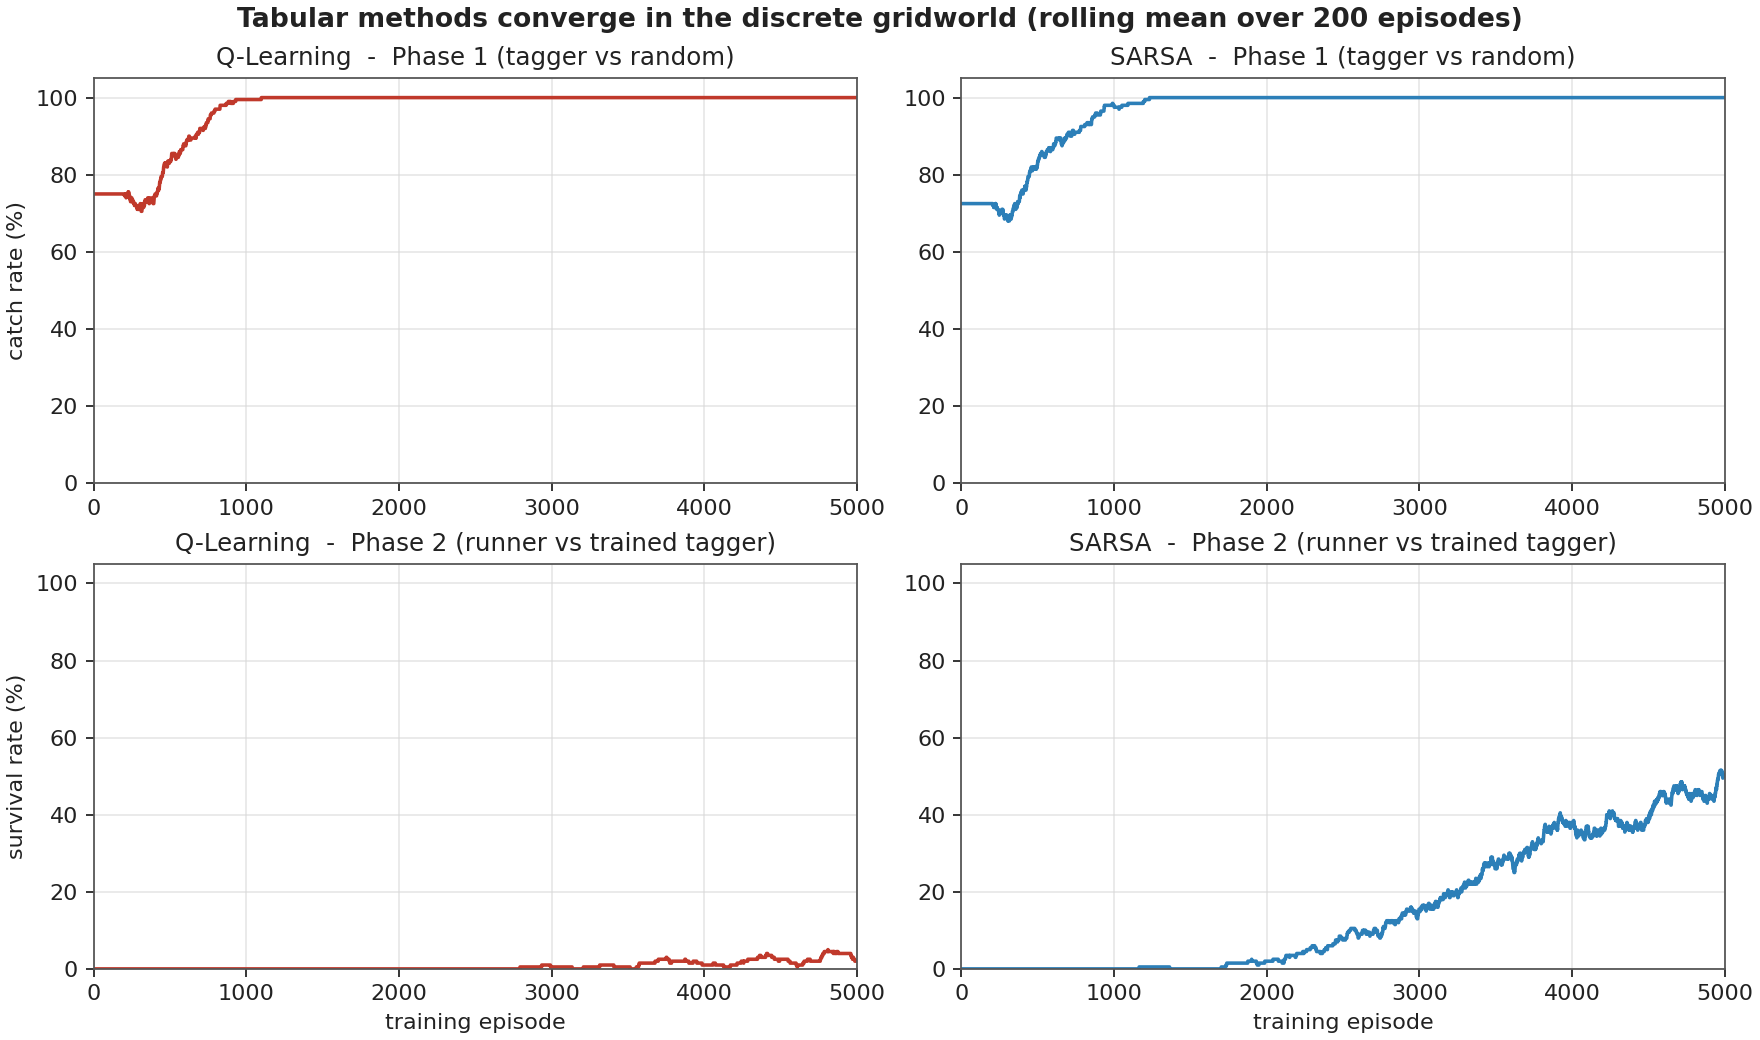
\includegraphics[width=0.92\columnwidth]{tabular_training_curves.png}}
\caption{Per-episode rolling means (window 200) for the two tabular
algorithms during Phase 1 and Phase 2 of gridworld training.}
\label{fig:tabular-training-curves}
\end{figure}

\textbf{Phase 3 (head-to-head).} The four algorithms produce four
qualitatively different equilibria. DQN is now the strongest evader of
the four: only 3.4\% of episodes end with a tag, and the average
episode length is 193.2 turns---essentially saturating the 200-turn
timeout. The DQN runner has internalized the same lesson that the
strong Phase-2 number predicted: against a frozen DQN tagger trained
only on a random opponent, the DQN runner reliably escapes for almost
the entire horizon. Q-Learning is second-most decisive on the tagger
side (62.5\% catch / 81.3 turns), consistent with its weak Phase-2
runner. SARSA produces the strongest stalemate signature (9.0\% catch
/ 182.7 turns): the SARSA tagger has not learned to chase a
stationary opponent, and the safety-first SARSA runner does not
provoke movement either. PPO is the opposite extreme of DQN: 100\% of
episodes end with a tag in an average of only 9.1 turns. The PPO
\emph{tagger} from Phase 1 is competent, but the PPO runner from
Phase 2 never learned an evasion policy at all, so the head-to-head
collapses into one-sided pursuit. Phase 3 thus inherits Phase 2's
sample-efficiency story directly: where Phase 2 produced a strong
runner (DQN, SARSA), Phase 3 produces long episodes; where Phase 2
produced no runner (PPO), Phase 3 produces short pursuits.

\subsubsection{Cliff-Walking Signature in the Gridworld}\label{sec:res-cliff}

Fig.~\ref{fig:cliffwalking} sharpens the SARSA/Q-Learning contrast in
terms of per-episode return. In Phase 1 (left panel) the two algorithms
are essentially indistinguishable: both converge to an average return
of $\sim{+}6$ at the same rate. In Phase 2 (right panel) they diverge
sharply: SARSA's per-episode return rises to roughly $+13$ while
Q-Learning's plateaus near $+3$. This is the empirical Cliff-Walking
signature. SARSA's on-policy update bootstraps from the action that the
agent will actually take next (which, with $\epsilon > 0$, is sometimes
random), so the Bellman target reflects the cost of any exploratory
mis-step that drops the runner into the tagger's reach. Q-Learning's
off-policy update bootstraps from the greedy maximum and ignores the
exploration cost, so it learns a more aggressive runner that performs
well only if the policy is actually executed greedily---which during
training, with $\epsilon > 0$, it is not.

\begin{figure}[t]
\centerline{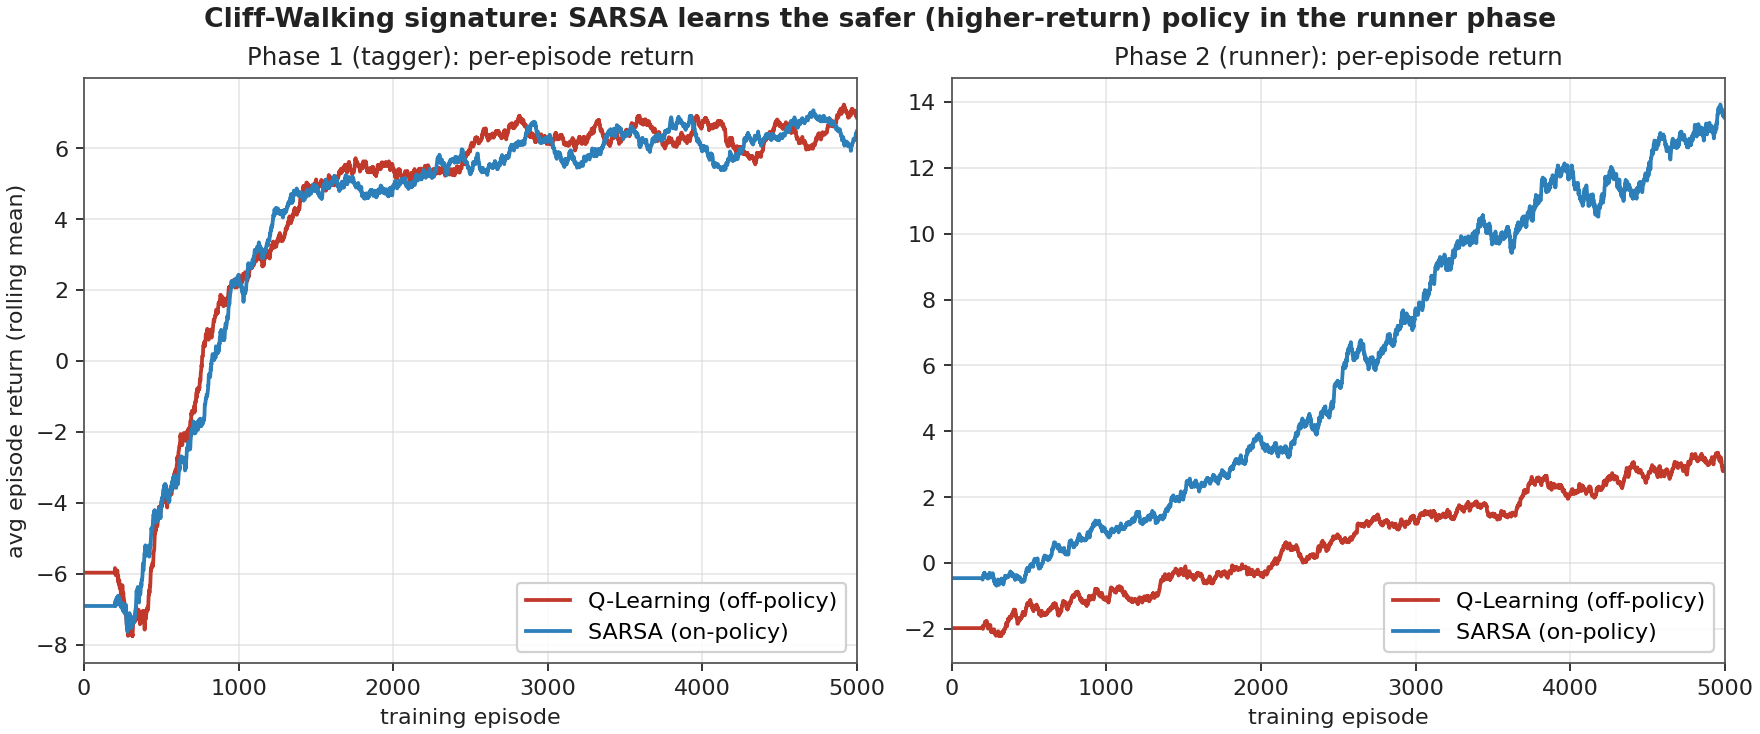
\includegraphics[width=0.92\columnwidth]{cliffwalking_risk_profile.png}}
\caption{Empirical Cliff-Walking signature in the gridworld. Average
per-episode return (rolling mean) during Phase 1 (left) and Phase 2
(right).}
\label{fig:cliffwalking}
\end{figure}


\subsection{Behavioral Observations}\label{sec:res-behavior}

We exported rendered evaluation videos for each checkpoint to
qualitatively inspect the moving patterns of each role. Trained taggers
consistently exhibit \emph{direct interception}, anticipating the
runner's heading rather than chasing the runner's current
position---an emergent behavior never explicitly rewarded. Runners
learn to \emph{wall-hug} when the tagger is far and to
\emph{break perpendicular} to the tagger's pursuit vector when close.
We also observed pathological patterns at low epochs: corner-camping
by runners (high reward at the cost of immobility) and stand-still
equilibria when both agents have weakly initialized Q-values. The
pure-proximity reward of Section~\ref{sec:reward} eliminates
corner-camping by making the danger penalty escalate quadratically
near the tagger, forcing motion. Fig.~\ref{fig:trajectory} overlays
the agent trajectories from a single evaluation episode of the
trained DQN policy at epoch 1000; runners trace clear arcs along the
room perimeter while the tagger converges on intercept points rather
than chasing through the centre.

\begin{figure}[t]
\centerline{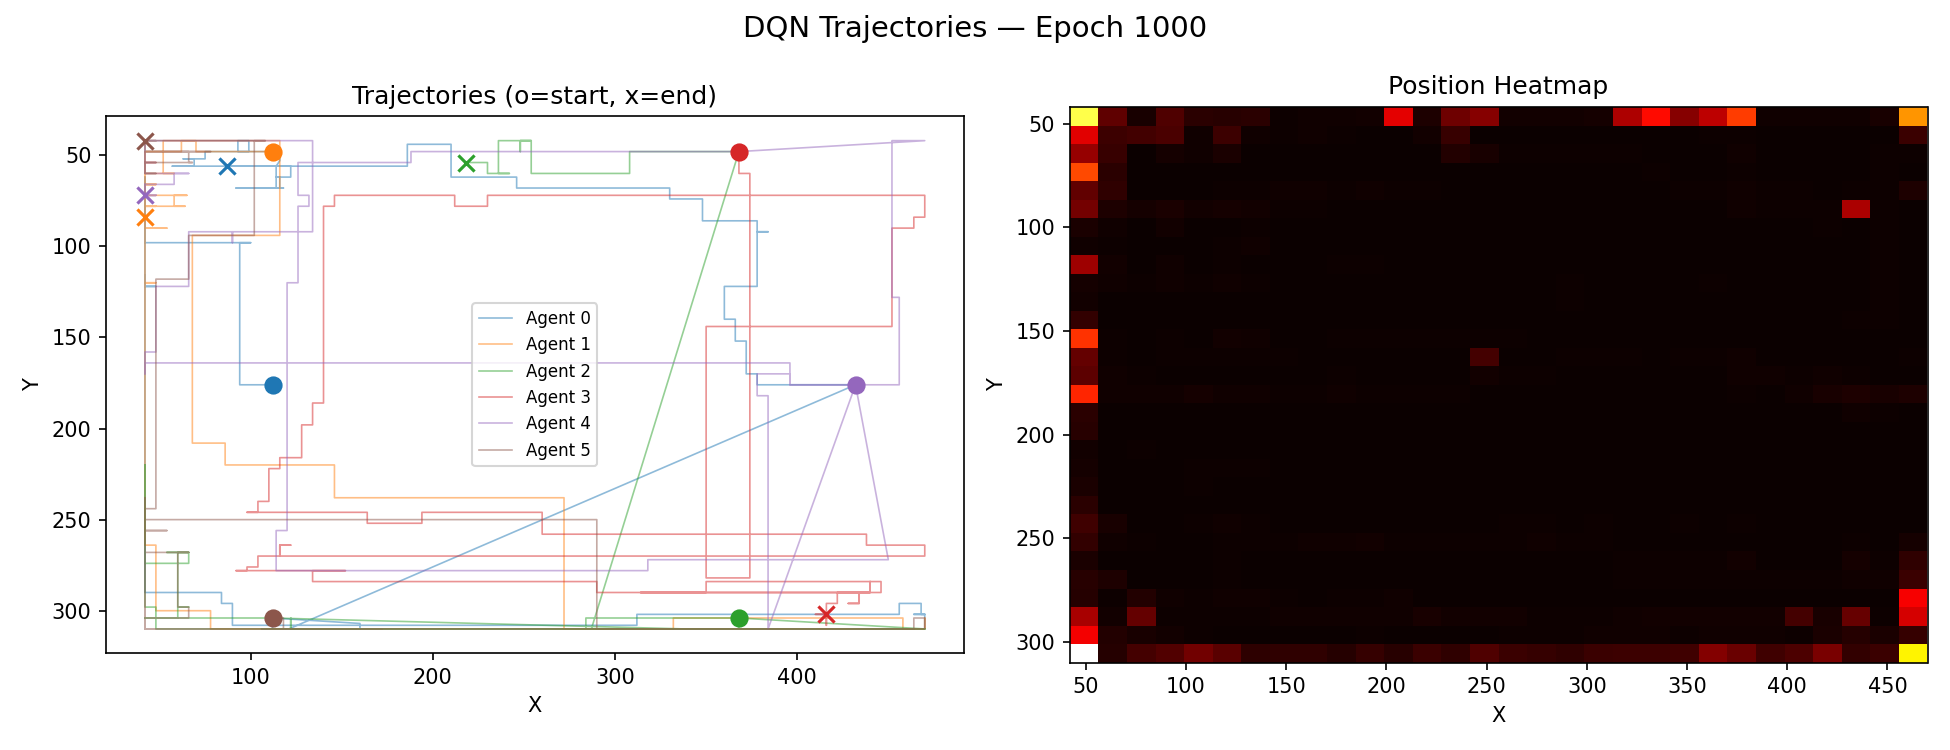
\includegraphics[width=0.95\columnwidth]{dqn_trajectory_1000.png}}
\caption{Agent trajectories from a single evaluation episode of the
trained DQN policy at epoch 1000.}
\label{fig:trajectory}
\end{figure}

\subsection{Why the Two Scenarios Diverge}\label{sec:res-synth}

The cleanest way to summarize the cross-scenario picture is to compare
Tables~\ref{tab:fullgame} and~\ref{tab:gridworld-all}. The tabular
methods produce zero tags in 1000 epochs of the continuous game and a
100\% catch rate in 5000 episodes of the gridworld. The deep methods
both succeed at Phase 1 in either scenario, but in the gridworld's
Phase 2 they split: DQN produces the single strongest runner of the
four algorithms (96.6\% survival), while PPO, with the same network
and hyperparameters, fails entirely (0\% survival). \emph{No single
algorithm wins across both scenarios, and within the gridworld no
single algorithm family wins both roles.} Three structural properties
of the task and the algorithms together explain the picture:

\begin{itemize}
    \item \textbf{State-space representation.} A Q-table indexed by
    discretized continuous observations is dominated by states that
    the agent never visits, so its $\hat Q(s,\cdot)$ is essentially
    untrained almost everywhere. Function approximators do not have
    this problem because they generalize across nearby observations.
    Consequently the continuous full game is tractable only for the
    deep methods, while the gridworld---with $10^4$ states---is also
    tractable for tabular methods, which inherit no disadvantage from
    the lack of generalization there.
    \item \textbf{Cliff-Walking risk profile (tabular).} Among the
    tabular methods, where both algorithms solve the chase task
    identically, the on-policy/off-policy distinction surfaces in the
    runner role: SARSA's on-policy update accounts for the cost of
    exploration and learns a safer (higher-return) runner;
    Q-Learning's off-policy update does not. \emph{On-policy wins
    among tabular.}
    \item \textbf{Sample efficiency under a fixed budget (deep).}
    Among the deep methods, the same on-policy/off-policy axis flips
    sign for a different reason. DQN reuses every transition through
    a 50k-capacity replay buffer, so each gradient step sees a mixture
    of recent and older experience; under our 5000-episode budget the
    runner converges to the strong evasion policy reported above. PPO
    is on-policy: each rollout is consumed in a handful of update
    epochs and then discarded, and with the same architecture and the
    same 5000-episode budget the runner network never accumulates
    enough policy-gradient signal to overcome the trained tagger.
    \emph{Off-policy wins among deep.}
\end{itemize}

The two within-family contrasts are interesting because they point in
\emph{opposite} directions on the on-policy/off-policy axis: SARSA
beats Q-Learning in the tabular runner role because on-policy targets
absorb exploration risk, but DQN beats PPO in the deep runner role
because off-policy replay extracts more learning from each trajectory.
The same algorithmic property is decisive in both scenarios; what
changes is which side of the property is the bottleneck. Combined with
the state-space axis, the result is a $2{\times}2$ scenario--family
pairing (tabular for discrete, deep for continuous) overlaid with a
role-specific learning-mechanism preference (on-policy for the safe
tabular runner, off-policy for the sample-hungry deep runner) rather
than a single best algorithm.

\section{Conclusion and Future Work}\label{sec:conclusion}

We built \textit{Learn To Tag} as a controlled comparison of four
standard RL algorithms (Q-Learning, SARSA, DQN, PPO) on two scenarios
that differ only in the structure of the state space: a continuous
2D Tag game and a $10{\times}10$ discrete gridworld. Three structural
properties---state representation, cliff-walking risk profile, and
sample efficiency under a fixed training budget---together shape
almost every result.

\textbf{State representation.} The full game's state is continuous, so
a Q-table indexed by binned observations is dominated by states the
agent never visits. Tabular methods cannot generalize across nearby
states and learn nothing (zero tags in 1000 epochs for both Q-Learning
and SARSA). Function approximators do not have this problem and learn
cleanly. The gridworld, with $10^4$ states, removes this obstacle and
all four algorithms learn at least a near-perfect tagger.

\textbf{Two-brain training.} Training a single network on both roles
produces conflicting gradients for the same observation. We sidestep
this by training every algorithm as two independent networks
($\pi_T$ for tagger, $\pi_R$ for runner) and reporting their
performance under an isolated-role protocol. Live runtime switching
between the two networks was part of our original design but is not
exercised in the experiments reported here; we revisit this in the
future-work list below.

\textbf{Headline findings.}
\begin{itemize}
    \item[(a)] All four algorithms train near-perfect \emph{taggers} in
    the $10{\times}10$ gridworld (99--100\% catch rate against a random
    runner), but the four algorithms diverge sharply on the runner
    role: DQN produces the strongest runner (96.6\% survival against a
    trained tagger), SARSA is second (89.4\%), Q-Learning is third
    (38.1\%), and PPO---trained with the same architecture and the
    same 5000-episode budget as DQN---fails entirely (0\% survival).
    \item[(b)] The SARSA-vs.-Q-Learning runner gap reproduces the
    classical Cliff-Walking risk-profile asymmetry, with SARSA's
    on-policy targets absorbing exploration risk where Q-Learning's
    off-policy targets do not. The DQN-vs.-PPO gap, in contrast,
    isolates a sample-efficiency effect: DQN's 50k-transition replay
    buffer reuses each transition many times, while PPO discards each
    rollout after a handful of update epochs. The two within-family
    contrasts therefore point in opposite directions on the
    on-policy/off-policy axis---on-policy wins among tabular,
    off-policy wins among deep---for two different mechanisms.
    \item[(c)] Phase~3 (head-to-head) inherits the Phase~2 picture.
    DQN produces the strongest evader of the four algorithms (only
    3.4\% catch rate, average episode length 193.2 turns, essentially
    saturating the 200-turn timeout); SARSA produces the strongest
    stalemate signature (9.0\% catch / 182.7 turns); Q-Learning is the
    most decisive tagger among the algorithms whose runner is weak
    (62.5\% catch); PPO collapses (100\% catch in 9.1 turns) because
    its runner network never learned an evasion policy. In the
    continuous full game PPO remains the stronger deep method, so
    neither deep algorithm dominates across both scenarios.
    \item[(d)] The tagger brain develops considerably faster than the
    runner brain across all deep runs---visible only because we report
    the two roles separately under the isolated-role protocol, and
    most extreme for PPO, whose tagger reaches 99.3\% catch rate while
    its runner never converges.
    \item[(e)] Iterative reward design showed that the simplest
    pure-proximity reward, with strong terminal events, was more
    reliable than every multi-term shaping function we tried before
    it. Each more elaborate variant introduced a distinct behavioural
    pathology (camping, oscillation, corner-hugging).
\end{itemize}

\textbf{Future work.}
\begin{itemize}
    \item[(i)] Implement the live two-brain wrapper at runtime so that
    a single agent can switch roles mid-episode in the continuous
    game, and re-evaluate joint performance with this routing in
    place.
    \item[(ii)] Filter eliminated entities out of the observation and
    reward computation so policies do not perceive or respond to
    inactive opponents.
    \item[(iii)] Further refine the reward function to suppress the
    near-timeout stalemates that emerge once both deep methods
    produce strong evaders.
    \item[(iv)] Cross-pair algorithms across roles---e.g., a Q-Learning
    tagger with a SARSA runner, or a PPO tagger with a DQN runner, in
    the gridworld---to exploit each algorithm's risk profile and
    sample-efficiency profile separately.
    \item[(v)] Re-run PPO under a much larger training budget (or
    with a heavier per-rollout update schedule) to test whether its
    gridworld runner role is recoverable in principle, separating the
    sample-efficiency story from any deeper algorithmic limitation.
    \item[(vi)] Run a curriculum across the small, medium, and large
    maps, transferring weights between phases, and increase the seed
    count for the deep-method comparison.
\end{itemize}

\begin{thebibliography}{00}
\bibitem{watkins1989} C.~J.~C.~H.~Watkins, ``Learning from Delayed Rewards,'' Ph.D. dissertation, Cambridge University, 1989.
\bibitem{rummery1994} G.~A.~Rummery and M.~Niranjan, ``On-line Q-learning using connectionist systems,'' Cambridge University Engineering Dept., Tech. Rep. CUED/F-INFENG/TR 166, 1994.
\bibitem{sutton2018} R.~S.~Sutton and A.~G.~Barto, \emph{Reinforcement Learning: An Introduction}, 2nd ed.\ \ \ Cambridge, MA: MIT Press, 2018. \url{http://incompleteideas.net/book/the-book-2nd.html}
\bibitem{mnih2015} V.~Mnih \emph{et al.}, ``Human-level control through deep reinforcement learning,'' \emph{Nature}, vol.~518, no.~7540, pp.~529--533, 2015. \url{https://doi.org/10.1038/nature14236}
\bibitem{schulman2017} J.~Schulman, F.~Wolski, P.~Dhariwal, A.~Radford, and O.~Klimov, ``Proximal policy optimization algorithms,'' arXiv:1707.06347, 2017. \url{https://arxiv.org/abs/1707.06347}
\bibitem{yu2022} C.~Yu \emph{et al.}, ``The Surprising Effectiveness of PPO in Cooperative Multi-Agent Games,'' in \emph{Proc.\ NeurIPS Datasets and Benchmarks}, 2022. \url{https://arxiv.org/abs/2103.01955}
\bibitem{baker2020} B.~Baker \emph{et al.}, ``Emergent Tool Use From Multi-Agent Autocurricula,'' in \emph{Proc.\ ICLR}, 2020. \url{https://arxiv.org/abs/1909.07528}
\bibitem{vanhasselt2016} H.~van~Hasselt, A.~Guez, and D.~Silver, ``Deep reinforcement learning with double Q-learning,'' in \emph{Proc.\ AAAI}, 2016. \url{https://arxiv.org/abs/1509.06461}
\bibitem{schaul2015} T.~Schaul, D.~Horgan, K.~Gregor, and D.~Silver, ``Universal value function approximators,'' in \emph{Proc.\ ICML}, 2015. \url{https://proceedings.mlr.press/v37/schaul15.html}
\bibitem{andreas2017} J.~Andreas, D.~Klein, and S.~Levine, ``Modular multitask reinforcement learning with policy sketches,'' in \emph{Proc.\ ICML}, 2017. \url{https://arxiv.org/abs/1611.01796}
\bibitem{wang2016} Z.~Wang, T.~Schaul, M.~Hessel, H.~van~Hasselt, M.~Lanctot, and N.~de~Freitas, ``Dueling network architectures for deep reinforcement learning,'' in \emph{Proc.\ ICML}, 2016. \url{https://arxiv.org/abs/1511.06581}
\bibitem{hessel2018} M.~Hessel \emph{et al.}, ``Rainbow: Combining improvements in deep reinforcement learning,'' in \emph{Proc.\ AAAI}, 2018. \url{https://arxiv.org/abs/1710.02298}
\bibitem{williams1992} R.~J.~Williams, ``Simple statistical gradient-following algorithms for connectionist reinforcement learning,'' \emph{Machine Learning}, vol.~8, no.~3--4, pp.~229--256, 1992. \url{https://doi.org/10.1007/BF00992696}
\bibitem{schulman2015} J.~Schulman, S.~Levine, P.~Moritz, M.~I.~Jordan, and P.~Abbeel, ``Trust region policy optimization,'' in \emph{Proc.\ ICML}, 2015. \url{https://arxiv.org/abs/1502.05477}
\bibitem{lowe2017} R.~Lowe, Y.~Wu, A.~Tamar, J.~Harb, P.~Abbeel, and I.~Mordatch, ``Multi-agent actor-critic for mixed cooperative-competitive environments,'' in \emph{Proc.\ NeurIPS}, 2017. \url{https://arxiv.org/abs/1706.02275}
\bibitem{rashid2018} T.~Rashid, M.~Samvelyan, C.~Schroeder~de~Witt, G.~Farquhar, J.~Foerster, and S.~Whiteson, ``QMIX: Monotonic value function factorisation for deep multi-agent reinforcement learning,'' in \emph{Proc.\ ICML}, 2018. \url{https://arxiv.org/abs/1803.11485}
\bibitem{terry2021} J.~K.~Terry \emph{et al.}, ``PettingZoo: Gym for multi-agent reinforcement learning,'' in \emph{Proc.\ NeurIPS}, 2021. \url{https://arxiv.org/abs/2009.14471}
\bibitem{liang2023} L.~Liang \emph{et al.}, ``Collaborative pursuit-evasion game of multi-UAVs based on Apollonius circle in the environment with obstacles,'' \emph{Connection Science}, vol.~35, no.~1, 2023. \url{https://doi.org/10.1080/09540091.2023.2168253}
\bibitem{kouzeghar2023} M.~Kouzeghar, Y.~Song, M.~Meghjani, and R.~Bouffanais, ``Multi-target pursuit by a decentralized heterogeneous UAV swarm using deep multi-agent reinforcement learning,'' in \emph{Proc.\ IEEE ICRA}, 2023. \url{https://arxiv.org/abs/2303.01799}
\bibitem{silver2017} D.~Silver \emph{et al.}, ``Mastering the game of Go without human knowledge,'' \emph{Nature}, vol.~550, no.~7676, pp.~354--359, 2017. \url{https://doi.org/10.1038/nature24270}
\bibitem{vinyals2019} O.~Vinyals \emph{et al.}, ``Grandmaster level in StarCraft II using multi-agent reinforcement learning,'' \emph{Nature}, vol.~575, no.~7782, pp.~350--354, 2019. \url{https://doi.org/10.1038/s41586-019-1724-z}
\bibitem{berner2019} C.~Berner \emph{et al.}, ``Dota 2 with large scale deep reinforcement learning,'' arXiv:1912.06680, 2019. \url{https://arxiv.org/abs/1912.06680}
\bibitem{wisniewski2024} M.~Wisniewski \emph{et al.}, ``Benchmarking deep reinforcement learning for navigation in denied sensor environments,'' arXiv:2410.14616, 2024. \url{https://arxiv.org/abs/2410.14616}
\end{thebibliography}

\end{document}
